\documentclass[11pt]{article}
\usepackage[a4paper,margin=2.5cm]{geometry}
\usepackage{amsmath,amssymb,amsthm,graphicx,booktabs,xcolor}
\usepackage[colorlinks=true,linkcolor=blue!60!black,citecolor=blue!60!black,urlcolor=blue!60!black]{hyperref}
\hypersetup{pdftitle={Multifractal Large Deviations in Quantum Entanglement},pdfauthor={Ruqing Chen}}

\newtheorem{theorem}{Theorem}
\newtheorem{proposition}{Proposition}[section]
\newtheorem{corollary}{Corollary}[section]
\newtheorem{lemma}{Lemma}[section]
\theoremstyle{definition}\newtheorem{definition}{Definition}[section]
\theoremstyle{remark}\newtheorem*{remark}{Remark}

\setlength{\emergencystretch}{2em}
\graphicspath{{../figures/}{figures/}{./}}
\newcommand{\dd}{\mathrm{d}}
\newcommand{\Tr}{\mathrm{Tr}}
\newcommand{\cL}{\mathcal{L}}
\newcommand{\GN}{G_N}

\title{Multifractal Large Deviations in Quantum Entanglement:\\
Ideal Fermi-Gas Mapping, Markov Tensor Cascades,\\ and Quartic Casimir Symmetry}
\author{Ruqing Chen\\[2pt]
\small GUT Geoservice Inc., Montreal, Quebec, Canada\\
\small \href{mailto:ruqing@hotmail.com}{\texttt{ruqing@hotmail.com}}}
\date{\small DOI: \href{https://doi.org/10.5281/zenodo.23193512}{10.5281/zenodo.23193512}}

\begin{document}
\maketitle

\begin{abstract}
The thermodynamic formalism of multifractals assigns to any normalised distribution a mass exponent
$\tau(q)$ and a singularity spectrum $f(\alpha)$. Applied to the eigenvalues of a reduced density matrix,
this formalism turns R\'enyi entropies into generalised dimensions and the refined R\'enyi entropy into
$f(\alpha_q)$. We use it to compare two notions that are often conflated: the multifractality of
single-particle wave functions at localisation transitions, and the multifractal structure of many-body
entanglement spectra.

For Gaussian fermionic states we prove that the refined R\'enyi entropy is exactly the entropy of an ideal
Fermi gas at temperature $1/q$ whose single-particle levels are the entanglement energies. The entanglement
singularity spectrum is therefore always non-negative and concave. Its dependence on wave-function
multifractality is mediated entirely by the density of entanglement energies, which is controlled by
inter-eigenstate overlaps rather than by single-state moments.

For tensor-network cascades with correlations between layers, modelled by a Markov chain, the mass exponent
is set by a Perron root. Its first-order correction is linear in the subleading eigenvalue $\lambda_2$, and it
is real-analytic for $\lambda_2<1$. A first-order (Maxwell) transition appears only in the reducible limit
$\lambda_2=1$.

At the quantum Hall transition, Weyl-group invariance makes the anomalous exponents functions of
$u=q(1-q)$. The measured non-parabolicity $b_1$ is then the coefficient of the $u^2$ (higher-Casimir) term.
This term appears at four loops in the $2+\varepsilon$ expansion with the same sign as observed, and its
non-vanishing excludes theories in which the relevant operators are current-algebra primaries of a WZW
model.

Finally, we compute Gauss--Bonnet cosmic branes in $d=4$. We confirm that the second Taylor coefficient of
$\tau(q)$ tracks $C_T/a$, find that the refined R\'enyi entropy turns negative at finite $q$ for positive
Gauss--Bonnet coupling, and explain why no correspondence between holographic couplings and the quantum Hall
coefficient $b_1$ should be expected.
\end{abstract}

\tableofcontents

%=====================================================================
\section{Introduction}
\label{sec:intro}

The multifractal formalism~\cite{Halsey,BeckSchlogl} describes a normalised measure $\{\mu_i\}$ on cells of
size $\varepsilon$ through the scaling of its moments, $\sum_i\mu_i^q\sim\varepsilon^{\tau(q)}$, and through
the Legendre transform $f(\alpha)=q\alpha-\tau(q)$, $\alpha=\tau'(q)$, which counts the cells with
$\mu_i\approx\varepsilon^{\alpha}$. The formalism is thermodynamic: $q$ plays the role of an inverse
temperature, $\tau$ of a free energy, $\alpha$ of an energy and $f$ of an entropy.

Two quite different physical objects are called ``multifractal'' in quantum many-body physics.
\begin{enumerate}
\item \emph{Wave-function multifractality.} At Anderson transitions and at the integer quantum Hall (IQH)
plateau transition, the single-particle probability $|\psi(r)|^2$ has moments
$\langle|\psi|^{2q}\rangle/\langle|\psi|^2\rangle^q\sim L^{-\Delta_q}$ with non-linear anomalous exponents
$\Delta_q$~\cite{EversMirlin}. The relevant measure lives on real space and is averaged over disorder.
\item \emph{Entanglement-spectrum multifractality.} The eigenvalues $\{\lambda_i\}$ of a reduced density
matrix $\rho_A$ form a normalised measure on the spectrum. Its moments are the R\'enyi entropies,
$S_q=\frac{1}{1-q}\ln\Tr\rho_A^q$. For a $1+1$-dimensional CFT the full eigenvalue density is the
Calabrese--Lefevre distribution~\cite{CL}.
\end{enumerate}
The same formalism applies to both, but the measures are different, and so are their symmetries and
positivity properties. Jia, Subramaniam, Gruzberg and Chakravarty showed that the summed single-site
entanglement of a single-particle critical state scales as $\alpha_1\ln L$~\cite{Jia}, a link through one
point of the spectrum only. Dong noted that the refined R\'enyi entropy is a thermodynamic entropy with respect
to the modular Hamiltonian~\cite{Dong}, which places the entanglement problem squarely within the
thermodynamic formalism.

\paragraph{Results.} Building on these works, we obtain the following.
\begin{enumerate}
\item \emph{Ideal Fermi-gas theorem} (Theorem~\ref{thm:fermi}). For any Gaussian fermionic state, the refined
R\'enyi entropy equals the entropy of an ideal Fermi gas at temperature $1/q$ with the entanglement energies as
single-particle levels. Consequently $f_{\rm ent}\ge0$ is concave and is fixed by the density of entanglement
energies. Wave-function multifractality enters only through that density, which depends on overlaps between
different eigenstates (Proposition~\ref{prop:nogo}).
\item \emph{Markov tensor cascades} (Section~\ref{sec:markov}). For layer-to-layer correlations modelled by a
Markov chain, $\tau(q)$ is a Perron root. Its correction is linear in $\lambda_2$, not a power $\lambda_2^q$,
and it is analytic for $\lambda_2<1$. Phase transitions require reducibility or quenched averaging.
\item \emph{Casimir structure at the IQH transition} (Section~\ref{sec:qh}). Writing the measured spectrum
in the Weyl-invariant variable $u=q(1-q)$ identifies $b_1$ with the coefficient of $u^2$. This term arises at
four loops in the $2+\varepsilon$ expansion, with the observed sign, and is incompatible with
current-algebra primaries of a WZW model.
\item \emph{Gauss--Bonnet cosmic branes} (Section~\ref{sec:holo}). The $q$-expansion of the holographic mass
exponent is controlled by CFT data such as $C_T/a$. Positive Gauss--Bonnet coupling leads to a negative refined
R\'enyi entropy at finite $q$. No dictionary between holographic couplings and $b_1$ is warranted.
\end{enumerate}
Section~\ref{sec:discussion} discusses limitations, and the Appendix collects numerical methods and
large-deviation derivations.

%=====================================================================
\section{Entanglement thermodynamics and the ideal Fermi-gas theorem}
\label{sec:fermi}

\subsection{The thermodynamic dictionary}
Let $\cL\to\infty$ be a large parameter, for instance $\cL=\ln(1/\varepsilon)$ or $\cL=\ln L$, and suppose
\begin{equation}
\ln\Tr\rho_A^q=-\tau(q)\,\cL+o(\cL)
\label{eq:tau}
\end{equation}
on an open interval $I$ of $q$ on which $\tau$ is differentiable.

\begin{proposition}[Thermodynamic dictionary]
\label{prop:dict}
Under~\eqref{eq:tau}, for $q\in I$,
\begin{align}
S_q&=D_q\,\cL+o(\cL),\qquad D_q=\frac{\tau(q)}{q-1},\\
\tilde S_q\equiv q^2\partial_q\Big(\frac{q-1}{q}S_q\Big)&=f(\alpha_q)\,\cL+o(\cL),\qquad
f(\alpha_q)=q\alpha_q-\tau(q),\qquad \alpha_q=\tau'(q),
\end{align}
and $\tilde S_q$ is the von Neumann entropy of the escort state $\rho_A^q/\Tr\rho_A^q$.
\end{proposition}
\begin{proof}
$\Phi(q)=\ln\Tr\rho_A^q$ is convex, being a log-sum-exp of functions linear in $q$. Pointwise convergence of
the convex functions $\Phi/\cL$ to a limit that is differentiable on $I$ implies convergence of their
derivatives~\cite[Thm.~25.7]{Rockafellar}. Since $\frac{q-1}{q}S_q=-\Phi/q$, we have
$\tilde S_q=\Phi-q\Phi'$, which converges to $(q\tau'-\tau)\cL$. For the escort state
$\pi_i=\lambda_i^q/\sum_j\lambda_j^q$, one finds $-\sum_i\pi_i\ln\pi_i=q\langle-\ln\lambda\rangle_\pi+\Phi=\Phi-q\Phi'$.
\end{proof}
Particular values have direct information-theoretic meaning: $D_0$ is the Hartley entropy (log-rank), $D_1$
the von Neumann entropy, $D_2$ the collision entropy, and $D_\infty=\alpha_{\min}$ the min-entropy, all per
unit $\cL$. Figure~\ref{fig:dict} illustrates the dictionary for a two-scale Cantor measure read as an
entanglement spectrum. There $\rho_A$ is either the exact cascade spectrum at finite resolution, or a tensor
product of $n$ ``bond'' qubits with Schmidt weights $(p_1,p_2)$. In the second case $S_q=n\,H_q(p)$ exactly, so
$D_q=H_q(p)/\ln2$.

\begin{figure}[t]
\centering
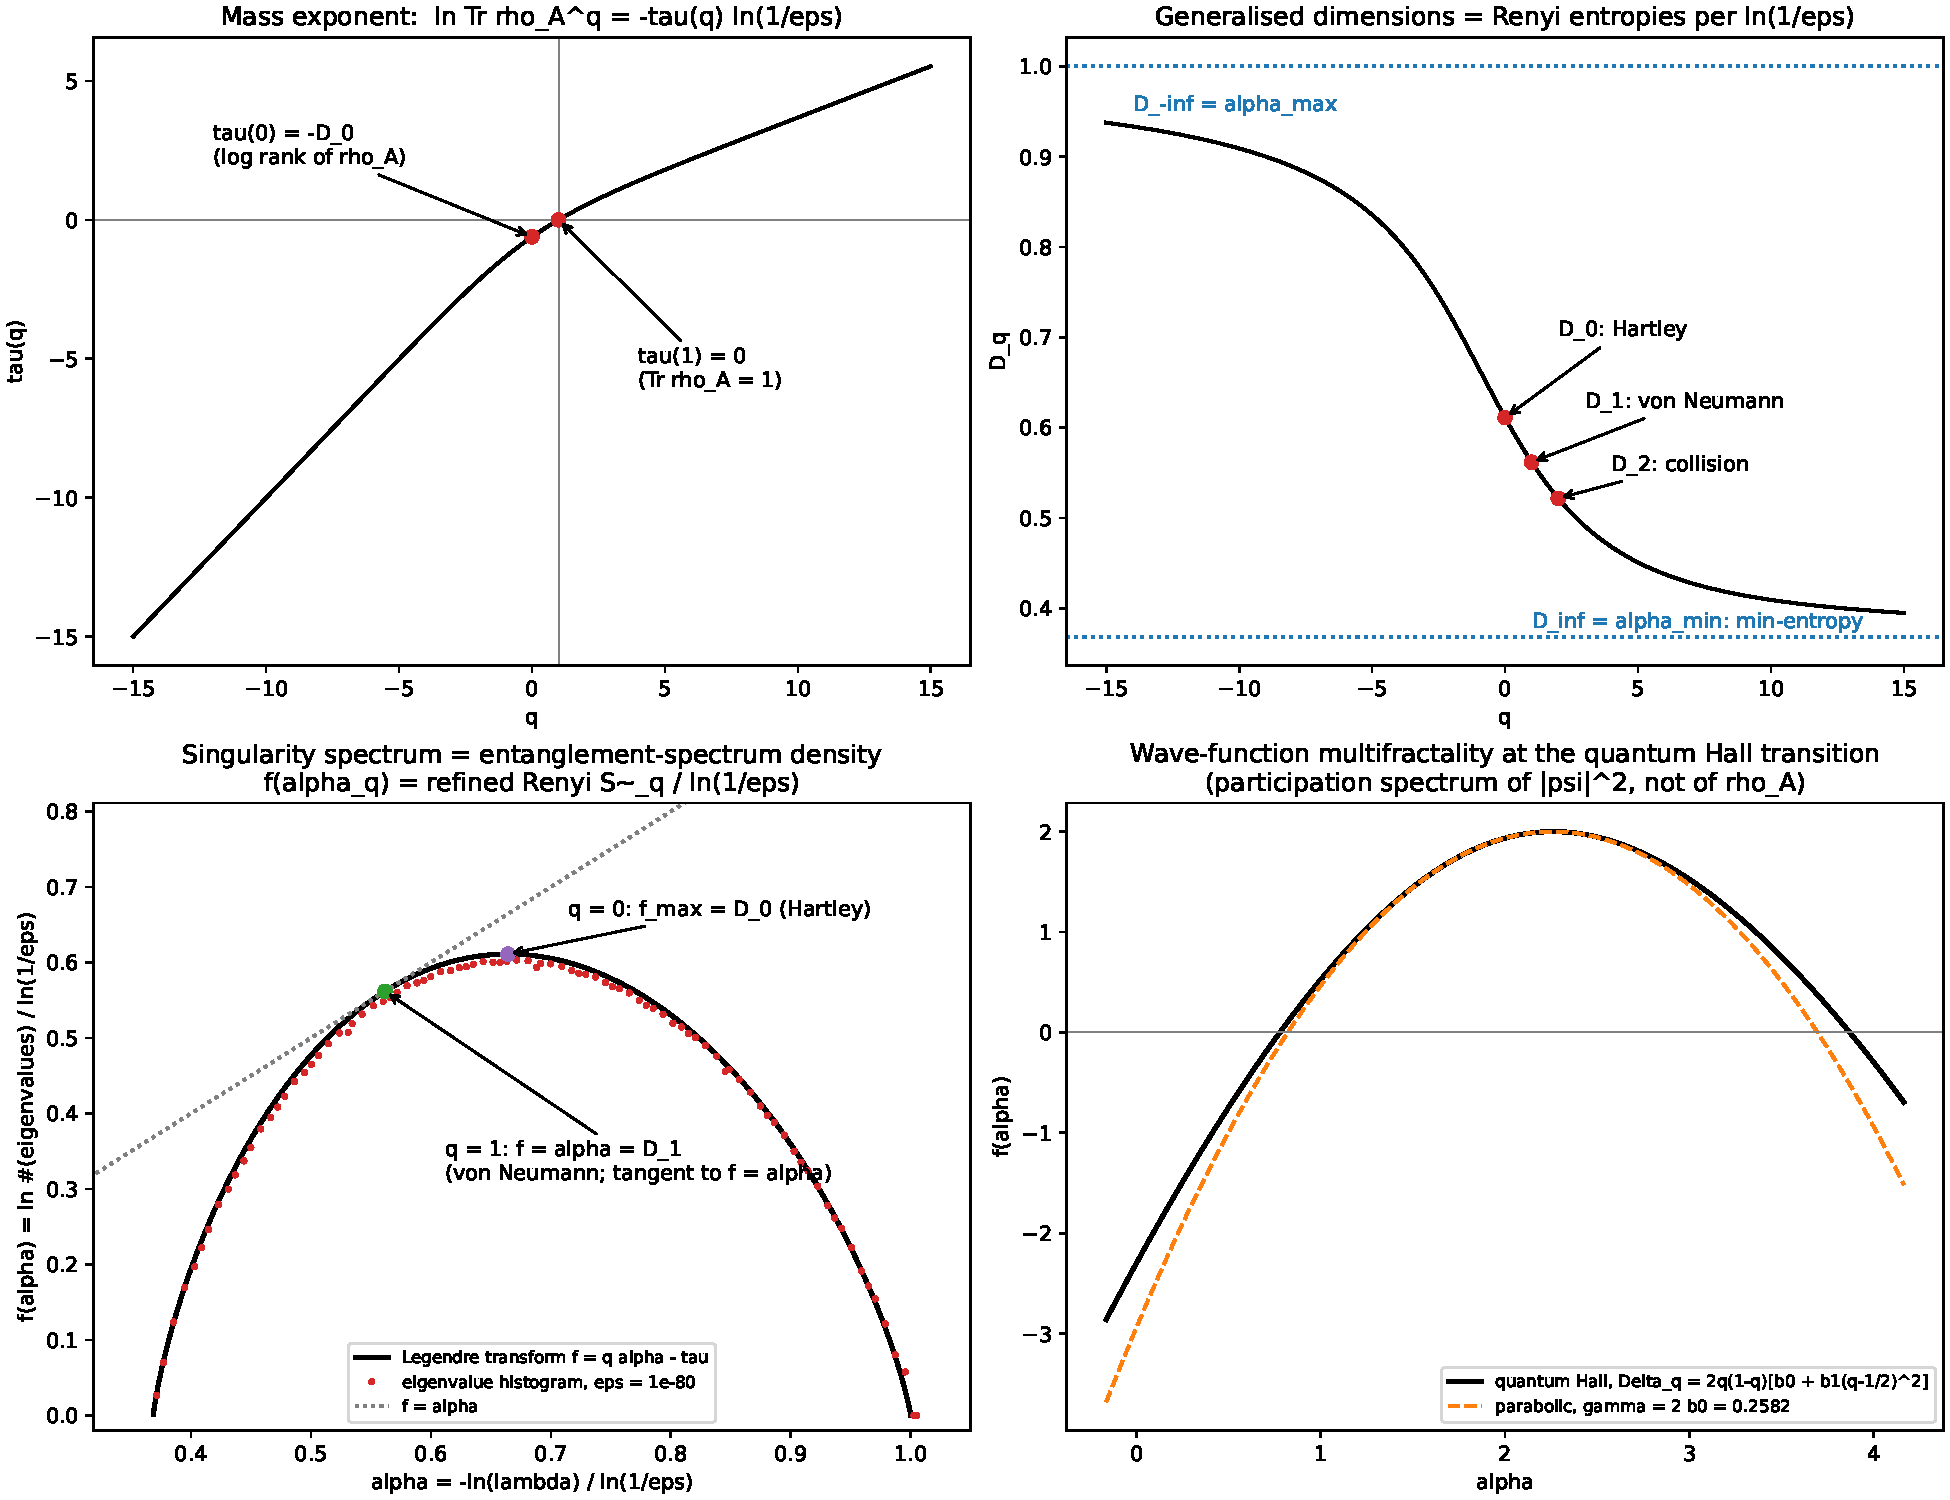
\includegraphics[width=\textwidth]{multifractal_entanglement}
\caption{Thermodynamic dictionary for a two-scale Cantor measure ($p=(0.6,0.4)$, $r=(0.25,0.4)$) read as
the eigenvalue distribution of $\rho_A$. Top left: mass exponent, with $\tau(0)=-D_0$ (log-rank) and
$\tau(1)=0$ (normalisation). Top right: generalised dimensions $D_q=S_q/\cL$, with the Hartley, von Neumann,
collision and min-entropies marked. Bottom left: singularity spectrum from the Legendre transform (line)
and from the exact eigenvalue histogram at $\varepsilon=10^{-80}$ (dots); the von Neumann point is tangent
to $f=\alpha$. Bottom right, for contrast: the quantum Hall wave-function spectrum
$\Delta_q=2q(1-q)[b_0+b_1(q-\tfrac12)^2]$ of~\cite{EMM} and its parabolic approximation. This is a
participation spectrum of $|\psi|^2$, not an entanglement spectrum.}
\label{fig:dict}
\end{figure}

\subsection{The ideal Fermi-gas theorem}
For a Gaussian fermionic state, Peschel's theorem~\cite{Peschel} gives
$\rho_A=Z^{-1}\exp(-\sum_k\varepsilon_k c_k^\dagger c_k)$. The entanglement energies $\varepsilon_k$ are related
to the eigenvalues $\zeta_k$ of the correlation matrix $C_{ij}=\langle c_i^\dagger c_j\rangle$, $i,j\in A$, by
$\zeta_k=(1+e^{\varepsilon_k})^{-1}$.

\begin{theorem}[Ideal Fermi-gas theorem]
\label{thm:fermi}
Let $\rho_A$ be Gaussian with entanglement energies $\{\varepsilon_k\}$, and set $n_q(\varepsilon)=(1+e^{q\varepsilon})^{-1}$
and $s_F(n)=-n\ln n-(1-n)\ln(1-n)$. Then, exactly,
\begin{align}
\ln\Tr\rho_A^q&=\sum_k\Big[\ln\big(1+e^{q\varepsilon_k}\big)-q\ln\big(1+e^{\varepsilon_k}\big)\Big],\label{eq:fermiZ}\\
\tilde S_q&=\sum_k s_F\big(n_q(\varepsilon_k)\big),\label{eq:fermiS}\\
\langle K\rangle_q&=\sum_k\Big[\ln\big(1+e^{\varepsilon_k}\big)-\varepsilon_k\big(1-n_q(\varepsilon_k)\big)\Big].\label{eq:fermiK}
\end{align}
In words, $\tilde S_q$ is the entropy of an ideal Fermi gas with single-particle levels $\varepsilon_k$ at
temperature $1/q$. If $\rho_A(\varepsilon)=\cL^{-1}\sum_k\delta(\varepsilon-\varepsilon_k)$ has a limit, then
$f_{\rm ent}(\alpha_q)=\int\dd\varepsilon\,\rho_A(\varepsilon)\,s_F(n_q(\varepsilon))$.
\end{theorem}
\begin{proof}
$\rho_A$ factorises over modes, with mode $k$ having eigenvalues $\zeta_k$ and $1-\zeta_k$, so
$\Tr\rho_A^q=\prod_k[\zeta_k^q+(1-\zeta_k)^q]$. With $\zeta=(1+e^{\varepsilon})^{-1}$ one has
$\zeta^q+(1-\zeta)^q=(1+e^{q\varepsilon})/(1+e^{\varepsilon})^q$, which gives~\eqref{eq:fermiZ}. The escort state
$\rho_A^q/\Tr\rho_A^q\propto\exp(-q\sum_k\varepsilon_kc_k^\dagger c_k)$ is Gaussian with occupations
$n_q(\varepsilon_k)$, and its von Neumann entropy is $\sum_ks_F(n_q)$; by Proposition~\ref{prop:dict} this is
$\tilde S_q$. Finally, $\langle K\rangle_q=-\partial_q\ln\Tr\rho_A^q$, which gives~\eqref{eq:fermiK}.
\end{proof}

\begin{corollary}
\label{cor:fermi}
(i) $f_{\rm ent}\ge0$ and $f_{\rm ent}$ is concave, as is any microcanonical entropy of an ideal gas.
(ii) $f_{\rm ent}$ depends on the state only through $\rho_A(\varepsilon)$. Each summand
in~\eqref{eq:fermiZ} is exactly invariant under $\varepsilon\to-\varepsilon$ (particle--hole exchange of a mode), so
$f_{\rm ent}$ depends only on the distribution of $|\varepsilon|$.
(iii) A uniform density $\rho_A(\varepsilon)=1/\pi^2$ per unit $\cL=\ln\ell$ gives, using
$\int_{\mathbb R}s_F\big((1+e^x)^{-1}\big)\dd x=\pi^2/3$,
\begin{equation}
f_{\rm ent}(\alpha_q)=\frac{1}{3q},
\end{equation}
which is the Calabrese--Lefevre result $f(\alpha_q)=c/(3q)$ with $c=1$~\cite{CL}.
\end{corollary}

\subsection{What wave-function multifractality can and cannot determine}
The correlation matrix of a Slater determinant is $C=P_A\Pi P_A$, where $\Pi=\sum_{n\in\rm occ}|\psi_n\rangle\langle\psi_n|$
and $P_A$ projects onto $A$. Its non-trivial spectrum coincides with that of the overlap matrix
$O_{nm}=\langle\psi_n|P_A|\psi_m\rangle$ restricted to occupied states.

\begin{proposition}[Structure of the map from wave functions to entanglement]
\label{prop:nogo}
\begin{enumerate}
\item[(i)] $f_{\rm ent}$ is a functional of the spectrum of $O$, i.e.\ of joint statistics of overlaps between
\emph{different} eigenstates. Single-state moments $\langle|\psi_n|^{2q}\rangle$, and hence $f_{\rm wave}$, do
not determine it. For example, the particle-number variance $\kappa_2=\Tr O(1-O)=\sum_{n\in\rm occ,\,m\notin\rm occ}
|\langle\psi_n|P_A|\psi_m\rangle|^2$, which controls the leading entanglement~\cite{KlichLevitov}, involves
cross-energy correlations.
\item[(ii)] There is no rescaling under which $f_{\rm ent}$ coincides with a disorder-averaged $f_{\rm wave}$ on
its full support. The latter can be negative and obeys $\Delta_q=\Delta_{1-q}$~\cite{MFME}, while
$f_{\rm ent}\ge0$ (Corollary~\ref{cor:fermi}) and $\tau_{\rm ent}$ has no $q\to1-q$ symmetry (for instance,
$\tau\propto q-1/q$ for a CFT).
\end{enumerate}
\end{proposition}
\begin{proof}
(i) follows from $\mathrm{spec}(P_A\Pi P_A)\setminus\{0\}=\mathrm{spec}(\Pi P_A\Pi)\setminus\{0\}$ and
Theorem~\ref{thm:fermi}. (ii) follows from the stated properties.
\end{proof}

\paragraph{Numerical test.} We diagonalised critical power-law random banded matrices (PRBM)~\cite{PRBM}
of the unitary class with $b=1$ and $N=2048$ (six realisations). We filled the lower half of the spectrum and
took $A$ to be half of the chain. The identity~\eqref{eq:fermiS} holds to a relative accuracy of
$5\times10^{-10}$. The wave-function spectrum of states near the band centre gives $D_2\simeq0.81$ and
$\alpha_0\simeq1.11$ at this size. The entanglement spectrum, normalised by $S_1=13.7$, is non-negative
everywhere, with minimum $0.026$, and departs visibly from the clean Calabrese--Lefevre form
(Fig.~\ref{fig:deep}, top left). Disorder thus changes $f_{\rm ent}$, but only through $\rho_A(\varepsilon)$, as
Theorem~\ref{thm:fermi} requires.

%=====================================================================
\section{Markov random cascades in tensor networks}
\label{sec:markov}

\subsection{From random tensor networks to cascades}
If a state can be written as $(V_A\otimes V_B)\bigotimes_{e\in\gamma}|\phi_e\rangle$ with isometries $V_A,V_B$ and bond
states $|\phi_e\rangle$ on a cut $\gamma$, then the non-zero spectrum of $\rho_A$ is that of
$\bigotimes_e\Tr_{\bar e}|\phi_e\rangle\langle\phi_e|$. For random tensor networks with large bond dimension, R\'enyi
entropies are given by sums of bond R\'enyi entropies along the minimal cut~\cite{HNQTWY}. For a
MERA-like network~\cite{Vidal}, the cut of an interval crosses a bounded number of bonds per layer over
$n\propto\log_bL$ layers. With identical bond spectra $\{p_j\}$, the spectrum of $\rho_A$ is then a multinomial
cascade, with
\begin{equation}
\tau(q)=-\frac{1}{\ln b}\ln\sum_jp_j^{\,q}\qquad(\text{per layer, }\cL=\ln L).
\end{equation}
The continuum $f(\alpha)$ arises from the discrete layers through Cram\'er's theorem: $\ln\lambda$ is a sum of
$n$ i.i.d.\ terms, and $f$ is the Legendre transform of their cumulant generating function (Appendix~\ref{app:ld}).
For a genuine MERA, disentanglers spoil the exact product structure, and the cascade is a model.

\subsection{Markov modulation}
To model residual correlations between layers, let the bond spectrum of layer $k$ depend on a sector $s_k$
that follows a Markov chain with transition matrix $T$ and stationary distribution $\pi$. Define
$z_q(s)=\sum_jp_{sj}^{\,q}$ and $D_q=\mathrm{diag}(z_q)$. The annealed partition function over $n$ layers is
$Z_n(q)=\pi^{\mathsf T}D_q(TD_q)^{n-1}\mathbf 1$.

\begin{proposition}[Perron-root mass exponent]
\label{prop:perron}
For irreducible aperiodic $T$, $\tau(q)=-\ln\Lambda_q/\ln b$, where $\Lambda_q$ is the Perron root of $TD_q$.
$\Lambda_q$ is real-analytic in $q$, so $\tau$ and $f$ have no singularities at finite $q$.
\end{proposition}
\begin{proof}
$TD_q$ is non-negative, irreducible and aperiodic, so its Perron root is simple and strictly dominant,
and $\frac1n\ln Z_n\to\ln\Lambda_q$. The
matrix entries are analytic in $q$, and a simple isolated eigenvalue of an analytic matrix family is
analytic~\cite{Kato}.
\end{proof}

\begin{proposition}[Two-state chain]
\label{prop:twostate}
For the symmetric two-state chain with second eigenvalue $\lambda_2$ and $\pi=(\tfrac12,\tfrac12)$, writing
$S=z_1+z_2$ and $P=z_1z_2$,
\begin{equation}
\Lambda_q=\tfrac14\Big[(1+\lambda_2)S+\sqrt{(1+\lambda_2)^2S^2-16\lambda_2P}\Big],
\end{equation}
\begin{equation}
\Delta\tau(q)\equiv\tau(q)-\tau(q)\big|_{\lambda_2=0}=-\frac{\lambda_2}{\ln b}\,\frac{\mathrm{Var}_\pi(z_q)}{\langle z_q\rangle_\pi^2}+O(\lambda_2^2).
\label{eq:dtau}
\end{equation}
\end{proposition}
\begin{proof}
With $T=\begin{pmatrix}1-e&e\\e&1-e\end{pmatrix}$ and $\lambda_2=1-2e$, the matrix $TD_q$ has trace
$\frac{1+\lambda_2}{2}S$ and determinant $\lambda_2P$, which gives the first formula. Differentiating at $\lambda_2=0$
gives $\partial_{\lambda_2}\Lambda_q=(z_1-z_2)^2/(2S)=\mathrm{Var}_\pi(z_q)/\langle z_q\rangle_\pi$.
\end{proof}
Two features distinguish~\eqref{eq:dtau} from a naive guess $\Delta\tau\propto\lambda_2^{\,q}$. The correction is
\emph{linear} in $\lambda_2$, because $\lambda_2$ weights a single transition per layer irrespective of $q$, and $q$
enters only through $\mathrm{Var}_\pi(z_q)$. Moreover $z_1(1)=z_2(1)=1$, so $\Delta\tau(1)=0$ and normalisation is
preserved.

\paragraph{Phase transitions.} By Proposition~\ref{prop:perron} there are none for $\lambda_2<1$. At $\lambda_2=1$
the chain is reducible and $\Lambda_q=\max(z_1,z_2)$. This has a kink wherever $z_1(q)=z_2(q)$ with different
slopes, and in particular at $q=1$ whenever the two sectors have different von Neumann entropies. The
Legendre transform then contains a linear segment, i.e.\ a Maxwell construction and a first-order transition.
For $\lambda_2\to1$ the discriminant shows that the crossover sharpens on the scale
$|z_1-z_2|\sim(1-\lambda_2)^{1/2}S$. Because the partition function is annealed over sectors, $f$ may become
negative, by the same mechanism that makes disorder-averaged wave-function spectra negative. A single
$\rho_A$ always has $f\ge0$.

\paragraph{Numerical test.} With bond spectra $(0.7,0.3)$ and $(0.9,0.1)$ and $b=2$, the first-order formula
reproduces the exact Perron result with relative error $2.1\times10^{-2}$ at $\lambda_2=0.05$ and $8.4\times10^{-2}$
at $\lambda_2=0.2$, i.e.\ with error $O(\lambda_2^2)$. A finite transfer-matrix product with $n=400$ layers gives
$0.6197$ against the Perron value $0.6194$ at $q=2.5$, $\lambda_2=0.5$. The sharpening of the crossover as
$\lambda_2\to1$ is shown in Fig.~\ref{fig:deep} (top right).

%=====================================================================
\section{Non-parabolicity and Casimir invariants at the quantum Hall critical point}
\label{sec:qh}

\subsection{Weyl invariance and the Casimir variable}
At Anderson transitions the multifractal exponents obey $\Delta_q=\Delta_{1-q}$~\cite{MFME}. Gruzberg,
Ludwig, Mirlin and Zirnbauer traced this symmetry to the invariance of the nonlinear $\sigma$-model under the
Weyl group of its target space~\cite{GLMZ}. Scaling operators are labelled by highest weights, and at one loop
their dimensions are proportional to the quadratic Casimir eigenvalue~\cite{GMZ}. For the operators
$|\psi|^{2q}$ the Weyl reflection acts as $q\to1-q$. Any Weyl-invariant function of $q$ is therefore a
function of
\begin{equation}
u=q(1-q).
\end{equation}

\begin{proposition}[Casimir form of the quantum Hall spectrum]
\label{prop:casimir}
The high-precision quantum Hall result~\cite{EMM},
$\Delta_q=2q(1-q)\big[b_0+b_1(q-\tfrac12)^2\big]$ with $b_0=0.1291\pm0.0002$ and $b_1=0.0029\pm0.0003$, is identical to
\begin{equation}
\Delta_q=c_1u+c_2u^2,\qquad c_1=2\big(b_0+\tfrac{b_1}{4}\big)=0.2596,\qquad c_2=-2b_1=-0.0058 .
\end{equation}
In particular $\alpha_0-2=\Delta'_0=c_1$, in agreement with the reported $\alpha_0=2.2596$.
\end{proposition}
\begin{proof}
Use $(q-\tfrac12)^2=\tfrac14-u$, which gives $2u[b_0+b_1(\tfrac14-u)]=2(b_0+\tfrac{b_1}4)u-2b_1u^2$. Also
$\Delta'_0=c_1$, since $u'(0)=1$ and $u(0)=0$.
\end{proof}
A parabolic spectrum is thus exactly the statement that $\Delta_q$ is linear in the quadratic Casimir. The
non-parabolicity $b_1$ measures the $u^2$ term, i.e.\ the contribution of higher Casimir invariants.

\subsection{Origin in the loop expansion}
In $2+\varepsilon$ dimensions the unitary-class result through four loops is~\cite{EversMirlin}
\begin{equation}
\Delta_q=q(1-q)\Big(\frac{\varepsilon}{2}\Big)^{1/2}-\frac38\,\zeta(3)\,q^2(q-1)^2\,\varepsilon^2+O(\varepsilon^{5/2})
=u\Big(\frac{\varepsilon}{2}\Big)^{1/2}-\frac38\zeta(3)\,u^2\varepsilon^2+\dots
\end{equation}
The $u^2$ term first appears at four loops, through the $\zeta(3)$ contribution. It gives $c_2=-\frac38\zeta(3)\varepsilon^2<0$,
that is,
\begin{equation}
b_1=\tfrac{3}{16}\zeta(3)\,\varepsilon^2>0,
\end{equation}
which has the same sign as the measured value. We stress that the $2+\varepsilon$ expansion is not controlled at
the IQH fixed point, which lies at strong coupling with topological angle $\theta=\pi$. The loop expansion
therefore explains the \emph{type} and \emph{sign} of the non-parabolic term, but not its magnitude.

\subsection{Incompatibility with current-algebra primaries}
\begin{proposition}
\label{prop:wzw}
If the operators $|\psi|^{2q}$ at the IQH fixed point were primaries of an affine current algebra realised
through the Sugawara construction (as in a WZW model), their dimensions would be proportional to the quadratic
Casimir, and $b_1$ would vanish.
\end{proposition}
\begin{proof}
For current-algebra primaries in a representation $R$, the Sugawara construction gives
$h_R=C_2(R)/(k+h^\vee)$~\cite{DiFrancesco}. The dimension is then a linear function of $C_2$, hence of $u$, and
$c_2=0$.
\end{proof}
Since $b_1=0.0029\pm0.0003$ differs from zero by about ten standard deviations~\cite{EMM}, theories in which the
multifractal operators are Sugawara primaries are excluded. This does not exclude a WZW model perturbed by an
operator that breaks the current algebra, nor a description in which $|\psi|^{2q}$ are not current-algebra
primaries. We do not know which operator generates the $u^2$ term at the IQH fixed point.

%=====================================================================
\section{Holographic duals and higher-curvature constraints}
\label{sec:holo}

\subsection{Cosmic branes and the two-dimensional case}
In holographic CFTs the refined R\'enyi entropy is the area of a cosmic brane of tension
$T_q=(q-1)/(4q\GN)$~\cite{Dong}. For spherical regions the brane is the horizon of a hyperbolic black hole at
temperature $T_0/q$~\cite{HMSY}. In $d=2$ the $q$-dependence of R\'enyi entropies is universal for every CFT,
$S_q=\frac c6(1+\frac1q)\ln(\ell/\varepsilon)$. The corresponding spectrum is
$f(\alpha)=\sqrt{\frac c3(2\alpha-\frac c3)}$~\cite{CL}, which is of square-root type rather than parabolic and has
no maximum: $\alpha\to\infty$ as $q\to0$. In a three-dimensional bulk the Gauss--Bonnet term vanishes
identically, so higher-curvature terms of this type cannot change the two-dimensional result.

\subsection{Gauss--Bonnet branes in $d=4$}
For Gauss--Bonnet gravity in $d+1=5$ dimensions, define $a=\lambda_{\rm GB}f_\infty=\frac12(1-\sqrt{1-4\lambda_{\rm GB}})$.
The temperature and horizon entropy of the hyperbolic black hole with horizon radius $x$, in units of the AdS
radius~\cite{Cai}, are
\begin{equation}
\frac{T(x)}{T_0}=\frac{d(1-a)x^4-(d-2)x^2+(d-4)a}{2x(x^2-2a)},\qquad
\frac{S(x)}{S_1}=x^{d-1}\,\frac{1-\frac{2a(d-1)}{(d-3)x^2}}{1-\frac{2a(d-1)}{d-3}} .
\end{equation}
Here $S(x)$ is the Jacobson--Myers horizon entropy, which replaces the area in Dong's prescription for this
theory~\cite{DongHD}. The brane sits at $x_q$, defined by $T(x_q)/T_0=1/q$. Define
$I(q)=\int_{x_q}^{1}\frac{S}{S_1}\,\dd\big(\frac{T}{T_0}\big)$. The thermodynamic method of~\cite{HMSY} then gives, exactly,
\begin{equation}
\tau(q)=q\,I(q),\qquad \alpha_q=I(q)+\frac{S(x_q)}{q\,S_1},\qquad f(\alpha_q)=\frac{S(x_q)}{S_1},
\end{equation}
in units of $S_1$. The last relation is Dong's formula, which is automatic in this construction.

\paragraph{$C_T$ universality.} Writing $\tau(q)=(q-1)+t_2(q-1)^2+\dots$, Perlmutter's theorem~\cite{Perlmutter}
fixes $t_2$ in terms of $C_T$ relative to the normalisation of $S_1$. For Gauss--Bonnet gravity in $d=4$ one has
$C_T\propto1-2a$ and $a_{\rm anom}\propto1-6a$~\cite{MyersSinha}, so
$t_2^{\rm GB}/t_2^{\rm E}=(1-2a)/(1-6a)$. Table~\ref{tab:gb} confirms this numerically to about $10^{-3}$. In the
Einstein limit, the numerically integrated $S_q$ agrees with the closed form of~\cite{HMSY} to
$3\times10^{-10}$.

\begin{table}[h]
\centering
\begin{tabular}{ccccc}
\toprule
$\lambda_{\rm GB}$ & $a$ & $t_2$ & $t_2/t_2^{\rm E}$ & $(1-2a)/(1-6a)$\\
\midrule
$-7/36$ & $-0.1667$ & $-0.3303$ & $0.6672$ & $0.6667$\\
$-0.10$ & $-0.0916$ & $-0.3782$ & $0.7639$ & $0.7635$\\
$0$ & $0$ & $-0.4951$ & $1$ & $1$\\
$0.05$ & $0.0528$ & $-0.6479$ & $1.3085$ & $1.3090$\\
$0.09$ & $0.1000$ & $-0.9895$ & $1.9985$ & $2.0000$\\
\bottomrule
\end{tabular}
\caption{Second Taylor coefficient of the holographic mass exponent for Gauss--Bonnet gravity in $d=4$,
over the allowed range $-7/36\le\lambda_{\rm GB}\le9/100$.}
\label{tab:gb}
\end{table}

\paragraph{Negative refined R\'enyi entropy at finite $q$.} For $a>0$ the Jacobson--Myers entropy changes sign
at $x^2=2a(d-1)/(d-3)$. As $q\to\infty$, $x_q^2\to(d-2)/(d(1-a))$ for $d=4$. At $\lambda_{\rm GB}=0.09$ we find that
$f(\alpha_q)=\tilde S_q/S_1$ becomes negative for $q>q_c\simeq6.47$ (Fig.~\ref{fig:deep}, bottom right). Because
$\tilde S_q$ is the entropy of a density matrix, it cannot be negative. The hyperbolic black-hole saddle
therefore cannot dominate beyond $q_c$, and another saddle, or a breakdown of the effective description, must
take over. This is a saddle-exchange transition of the kind discussed in Section~\ref{sec:markov}.

\subsection{No dictionary between $b_1$ and $\lambda_{\rm GB}$}
It is tempting to relate the quantum Hall coefficient $b_1$ to a holographic coupling such as
$\lambda_{\rm GB}$. We argue that this would be unfounded, for three reasons.
\begin{enumerate}
\item The measures differ: a disorder-averaged participation spectrum ($f$ may be negative,
$\Delta_q=\Delta_{1-q}$) versus the entanglement spectrum of a clean, strongly coupled CFT ($f\ge0$, no $q\to1-q$
symmetry).
\item The dimensions differ: the IQH transition is two-dimensional, where holographic R\'enyi entropies are
universal, whereas Gauss--Bonnet effects require $d\ge4$.
\item The Weyl-invariant variable $u$ that organises the quantum Hall spectrum has no counterpart in
$\tau_{\rm ent}$.
\end{enumerate}
What the two problems share is an organising principle. In each case the departure from the leading form is
controlled by the next invariant of the critical theory: the $u^2$ (higher-Casimir) term for localisation, and
CFT data such as $C_T/a$ and $\langle TTT\rangle$ for holography.

\begin{figure}[t]
\centering
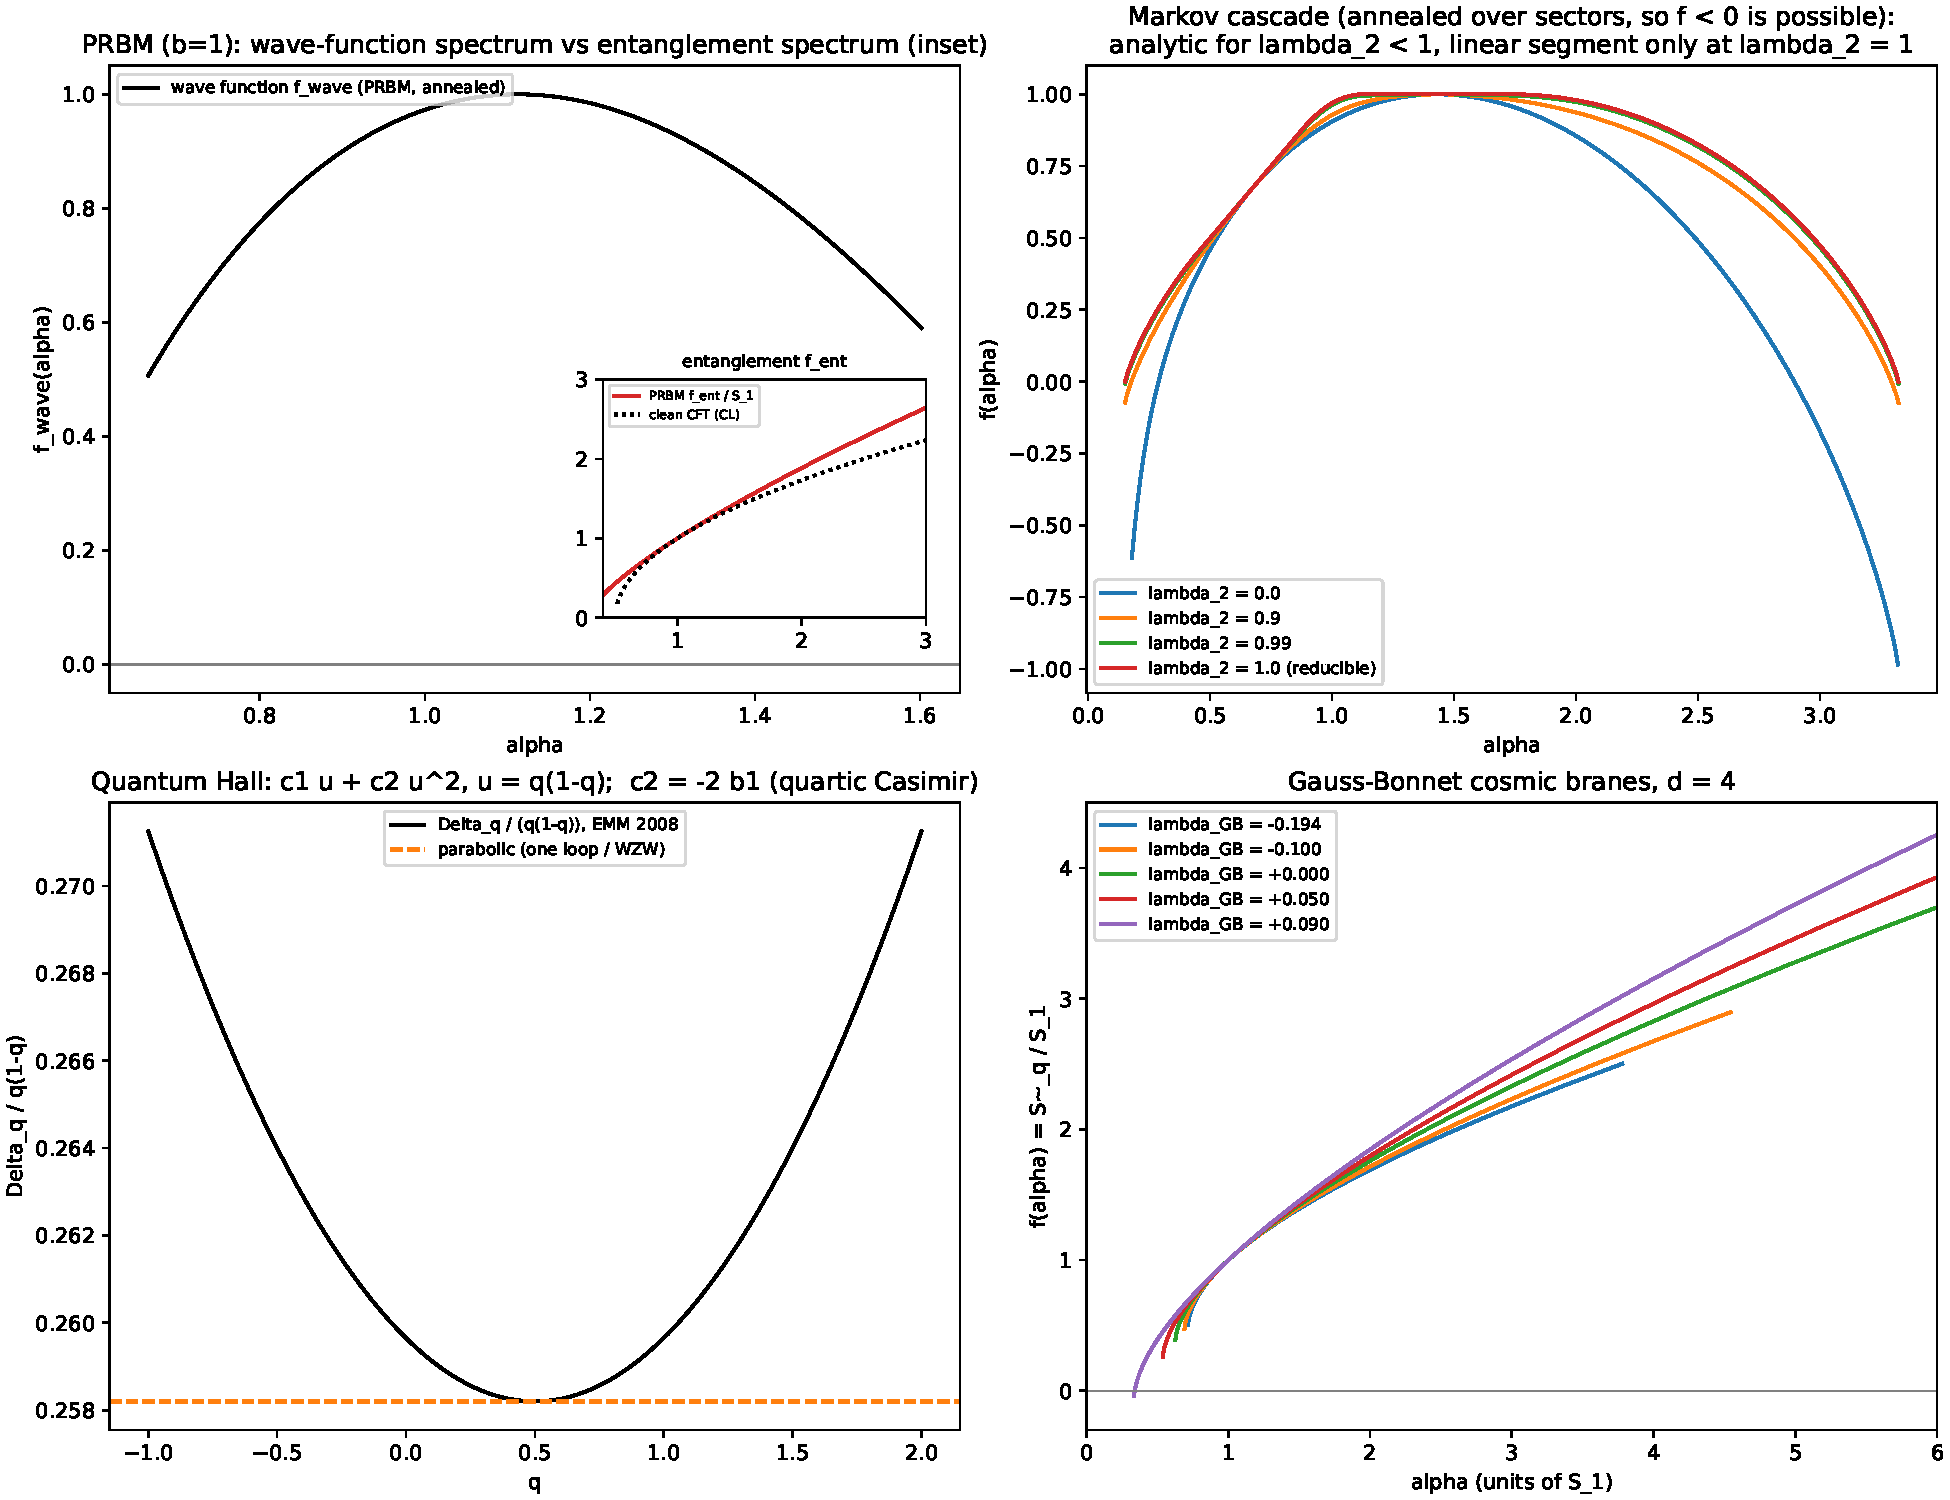
\includegraphics[width=\textwidth]{frontier2_deepdive}
\caption{Top left: wave-function singularity spectrum of a critical PRBM ($b=1$, $N=2048$, annealed over
states near the band centre); inset: entanglement spectrum $f_{\rm ent}/S_1$ of the half-filled Slater
determinant compared with the clean Calabrese--Lefevre form. Top right: Markov-modulated cascade, annealed
over sectors, for $\lambda_2=0,0.9,0.99,1$; the spectrum is analytic for $\lambda_2<1$ and develops a linear segment
at $\lambda_2=1$. Bottom left: quantum Hall $\Delta_q/q(1-q)$~\cite{EMM} against the parabolic value; the curvature is
the $u^2$ coefficient $c_2=-2b_1$. Bottom right: Gauss--Bonnet cosmic-brane spectra in $d=4$.}
\label{fig:deep}
\end{figure}

%=====================================================================
\section{Discussion and limitations}
\label{sec:discussion}
\begin{enumerate}
\item Theorem~\ref{thm:fermi} is exact but specific to Gaussian states. For interacting systems the modular
Hamiltonian is not quadratic, and $f_{\rm ent}$ is no longer an ideal-gas entropy.
\item Proposition~\ref{prop:nogo} is a structural statement. We have not derived $\rho_A(\varepsilon)$ from the
multi-state correlations of critical wave functions; doing so would require the joint statistics of
overlaps across energies, beyond the single-state exponents $\Delta_q$.
\item The PRBM numerics use a single system size, so the extracted exponents ($D_2\simeq0.81$, $\alpha_0\simeq1.11$)
carry finite-size corrections that we have not quantified.
\item The Markov cascade is a phenomenological model of residual inter-layer correlations in tensor
networks, and its partition function is annealed. Quenched (typical) averages may exhibit freezing-type
transitions that we have not analysed.
\item Section~\ref{sec:qh} identifies the type and sign of the non-parabolic term, but the $2+\varepsilon$
expansion is not controlled at the IQH fixed point. The operator generating the $u^2$ term remains unknown.
\item The negative refined R\'enyi entropy for $\lambda_{\rm GB}>0$ indicates a change of dominant saddle; we have not
constructed the competing saddle.
\end{enumerate}

\section*{Data and code availability}
All figures and numbers are produced by two Python scripts, \texttt{multifractal\_entanglement.py}
(Section~\ref{sec:fermi}, Fig.~\ref{fig:dict}) and \texttt{frontier2\_deepdive.py} (Sections~\ref{sec:fermi}--\ref{sec:holo},
Fig.~\ref{fig:deep}, Table~\ref{tab:gb}), available at
\url{https://github.com/Ruqing1963/multifractal-quantum-entanglement} and archived on Zenodo under DOI
\href{https://doi.org/10.5281/zenodo.23193512}{10.5281/zenodo.23193512}.

\appendix
\section{Numerical methods}
\label{app:numerics}
\begin{itemize}
\item \emph{Two-scale Cantor measure.} $\tau(q)$ is obtained from $\sum_ip_i^qr_i^{-\tau}=1$ by Brent's method, with
$\alpha=\sum_iw_i\ln p_i/\sum_iw_i\ln r_i$ and $w_i=p_i^qr_i^{-\tau}$. The exact spectrum at resolution $\varepsilon$ is
enumerated by composition $(k_1,k_2)$ with the stopping rule ``first prefix of size $\le\varepsilon$'', using logarithmic
binomial coefficients. The trace equals $1$ to $10^{-12}$. At $\varepsilon=10^{-80}$, $S_q/\cL$ differs from $D_q$ by
$O(1/\cL)$, e.g.\ $0.5633$ against $0.5616$ at $q=1$.
\item \emph{PRBM.} $H_{ij}$ is complex Gaussian with variance $[1+(r_{ij}/b)^2]^{-1}$, using the periodic distance
$r_{ij}$, and is Hermitised. $C$ is formed from the lower half of the eigenvectors. Wave-function moments use
box sizes $2,4,\dots,N/8$ and the 64 states closest to the band centre. Entanglement quantities use
$\ln(\zeta^q+(1-\zeta)^q)$ with $\zeta$ clipped to $[10^{-15},1-10^{-15}]$.
\item \emph{Markov cascade.} The Perron root is computed by dense diagonalisation of $TD_q$. The finite-$n$
check multiplies normalised row vectors for $n=400$ layers.
\item \emph{Gauss--Bonnet.} $x_q$ is found by Brent's method above the largest zero of the numerator of $T(x)$.
$I(q)$ is computed by adaptive quadrature, and $\alpha_q$ from the exact relation in Section~\ref{sec:holo}. $t_2$ is
obtained by central differences on a uniform grid in $q$.
\end{itemize}

\section{Large-deviation derivations}
\label{app:ld}
\paragraph{Equal-scale cascade (Cram\'er).} With $n$ independent layers and bond spectrum $\{p_j\}$, the
eigenvalues are $\lambda=\prod_kp_{j_k}$. Their number with $-\ln\lambda/(n\ln b)\in[\alpha,\alpha+\dd\alpha]$ is a multinomial
count. By Stirling's formula, or equivalently Cram\'er's theorem for the empirical frequencies~\cite{DemboZeitouni},
it behaves as $b^{nf(\alpha)}$, with $f$ the Legendre transform of $\tau(q)=-\log_b\sum_jp_j^q$.

\paragraph{Markov modulation (G\"artner--Ellis).} For an irreducible Markov additive process the scaled
cumulant generating function exists and equals $\ln\Lambda_q$, the logarithm of the Perron root of the tilted
matrix~\cite{DemboZeitouni}. Since it is differentiable, the G\"artner--Ellis theorem yields the large-deviation
rate function as its Legendre transform, which is $f$ up to normalisation.

\paragraph{Crossover width near $\lambda_2=1$.} For $\lambda_2=1-2e$ the discriminant in Proposition~\ref{prop:twostate}
is $4(z_1-z_2)^2+O(e)S^2$. The smooth $\Lambda_q$ therefore deviates from $\max(z_1,z_2)$ appreciably only where
$(z_1-z_2)^2\lesssim eS^2$, i.e.\ on a window of width $\propto(1-\lambda_2)^{1/2}$ around each crossing.

\begin{thebibliography}{99}
\bibitem{Halsey} T.~C.~Halsey, M.~H.~Jensen, L.~P.~Kadanoff, I.~Procaccia, B.~I.~Shraiman, ``Fractal measures and their singularities: The characterization of strange sets'', Phys.\ Rev.\ A 33 (1986) 1141.
\bibitem{BeckSchlogl} C.~Beck, F.~Schl\"ogl, \emph{Thermodynamics of Chaotic Systems: An Introduction}, Cambridge University Press (1993).
\bibitem{EversMirlin} F.~Evers, A.~D.~Mirlin, ``Anderson transitions'', Rev.\ Mod.\ Phys.\ 80 (2008) 1355, arXiv:0707.4378.
\bibitem{CL} P.~Calabrese, A.~Lefevre, ``Entanglement spectrum in one-dimensional systems'', Phys.\ Rev.\ A 78 (2008) 032329, arXiv:0806.3059.
\bibitem{Jia} X.~Jia, A.~R.~Subramaniam, I.~A.~Gruzberg, S.~Chakravarty, ``Entanglement entropy and multifractality at localization transitions'', Phys.\ Rev.\ B 77 (2008) 014208, arXiv:0710.1871.
\bibitem{Dong} X.~Dong, ``The gravity dual of R\'enyi entropy'', Nature Commun.\ 7 (2016) 12472, arXiv:1601.06788.
\bibitem{Rockafellar} R.~T.~Rockafellar, \emph{Convex Analysis}, Princeton University Press (1970).
\bibitem{EMM} F.~Evers, A.~Mildenberger, A.~D.~Mirlin, ``Multifractality at the quantum Hall transition: Beyond the parabolic paradigm'', Phys.\ Rev.\ Lett.\ 101 (2008) 116803, arXiv:0804.2334.
\bibitem{Peschel} I.~Peschel, ``Calculation of reduced density matrices from correlation functions'', J.\ Phys.\ A 36 (2003) L205.
\bibitem{KlichLevitov} I.~Klich, L.~Levitov, ``Quantum noise as an entanglement meter'', Phys.\ Rev.\ Lett.\ 102 (2009) 100502, arXiv:0804.1377.
\bibitem{MFME} A.~D.~Mirlin, Y.~V.~Fyodorov, A.~Mildenberger, F.~Evers, ``Exact relations between multifractal exponents at the Anderson transition'', Phys.\ Rev.\ Lett.\ 97 (2006) 046803, arXiv:cond-mat/0603378.
\bibitem{PRBM} A.~D.~Mirlin, Y.~V.~Fyodorov, F.-M.~Dittes, J.~Quezada, T.~H.~Seligman, ``Transition from localized to extended eigenstates in the ensemble of power-law random banded matrices'', Phys.\ Rev.\ E 54 (1996) 3221.
\bibitem{HNQTWY} P.~Hayden, S.~Nezami, X.-L.~Qi, N.~Thomas, M.~Walter, Z.~Yang, ``Holographic duality from random tensor networks'', JHEP 11 (2016) 009, arXiv:1601.01694.
\bibitem{Vidal} G.~Vidal, ``Entanglement renormalization'', Phys.\ Rev.\ Lett.\ 99 (2007) 220405.
\bibitem{Kato} T.~Kato, \emph{Perturbation Theory for Linear Operators}, Springer.
\bibitem{GLMZ} I.~A.~Gruzberg, A.~W.~W.~Ludwig, A.~D.~Mirlin, M.~R.~Zirnbauer, ``Symmetries of multifractal spectra and field theories of Anderson localization'', Phys.\ Rev.\ Lett.\ 107 (2011) 086403, arXiv:1103.4627.
\bibitem{GMZ} I.~A.~Gruzberg, A.~D.~Mirlin, M.~R.~Zirnbauer, ``Classification and symmetry properties of scaling dimensions at Anderson transitions'', Phys.\ Rev.\ B 87 (2013) 125144, arXiv:1210.6726.
\bibitem{DiFrancesco} P.~Di~Francesco, P.~Mathieu, D.~S\'en\'echal, \emph{Conformal Field Theory}, Springer (1997).
\bibitem{HMSY} L.-Y.~Hung, R.~C.~Myers, M.~Smolkin, A.~Yale, ``Holographic calculations of R\'enyi entropy'', JHEP 12 (2011) 047, arXiv:1110.1084.
\bibitem{Cai} R.-G.~Cai, ``Gauss--Bonnet black holes in AdS spaces'', Phys.\ Rev.\ D 65 (2002) 084014, arXiv:hep-th/0109133.
\bibitem{DongHD} X.~Dong, ``Holographic entanglement entropy for general higher derivative gravity'', JHEP 01 (2014) 044, arXiv:1310.5713.
\bibitem{Perlmutter} E.~Perlmutter, ``A universal feature of CFT R\'enyi entropy'', JHEP 03 (2014) 117, arXiv:1308.1083.
\bibitem{MyersSinha} R.~C.~Myers, A.~Sinha, ``Holographic c-theorems in arbitrary dimensions'', JHEP 01 (2011) 125, arXiv:1011.5819.
\bibitem{DemboZeitouni} A.~Dembo, O.~Zeitouni, \emph{Large Deviations Techniques and Applications}, 2nd ed., Springer (1998).
\end{thebibliography}
\end{document}
